\begin{figure}[H]
\begin{center}
  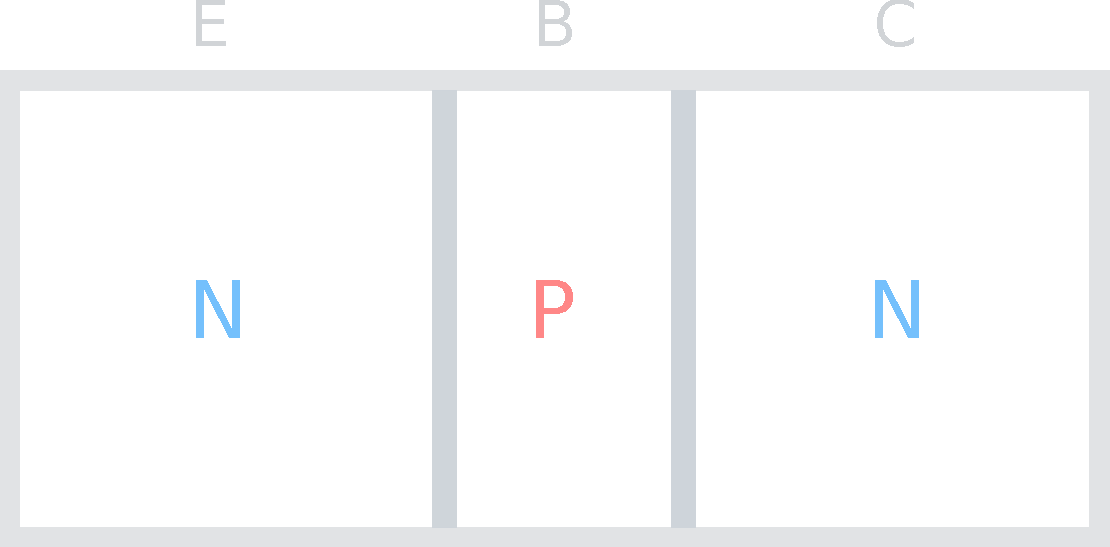
\includegraphics[width=0.618\textwidth]{1_1/npn.pdf}
  \end{center}
\end{figure}

Die Funktion des \emph{Bi}polartransistors basiert auf beiden Ladungsträger
-bzw. Halbleiterdotierungsarten. Je nach Transistortyp haben die drei Halbleitergebiete des Bipolartransistors die Dotierfolge NPN oder PNP, die einzelnen Regionen heißen Basis (B), Kollektor (C) und Emitter, welche unterschiedlich dotiert sind.\\

\begin{figure}[H]
\begin{center}
  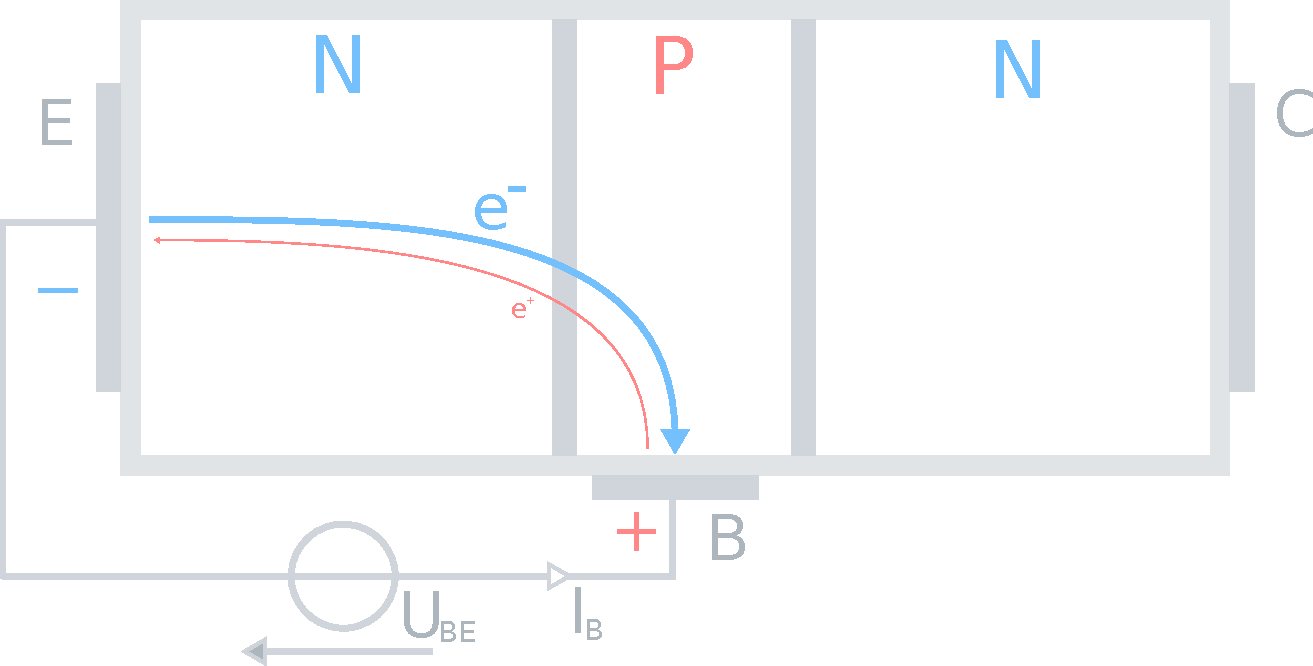
\includegraphics[width=0.618\textwidth]{1_1/npn_voltage.pdf}
  \end{center}
\end{figure}
Funktion am Beispiel des NPN-Transistors:
Ist die von außen anliegende Spannung $U_{\textrm{BE}}= 0\, \si{\volt}$, sind alle pn-Übergänge in Sperrrichtung und es fließt kein Strom durch den Transistor. Bei einer Spannung von etwa $U_{\textrm{BE}}=0.7\,\si{\volt}$ gerät der Basis-Emitter-Übergang in Durchlassrichtung. Löcher aus dem p-Gebiet (Basis) diffundieren in das n-Gebiet (Emitter) (vgl. Diode) und rekombinieren mit den dort befindlichen Leitungselektronen. Umgekehrt diffundieren die Elektronen des Emitters ebenfalls in die Basis. \\

\begin{figure}[H]
\begin{center}
  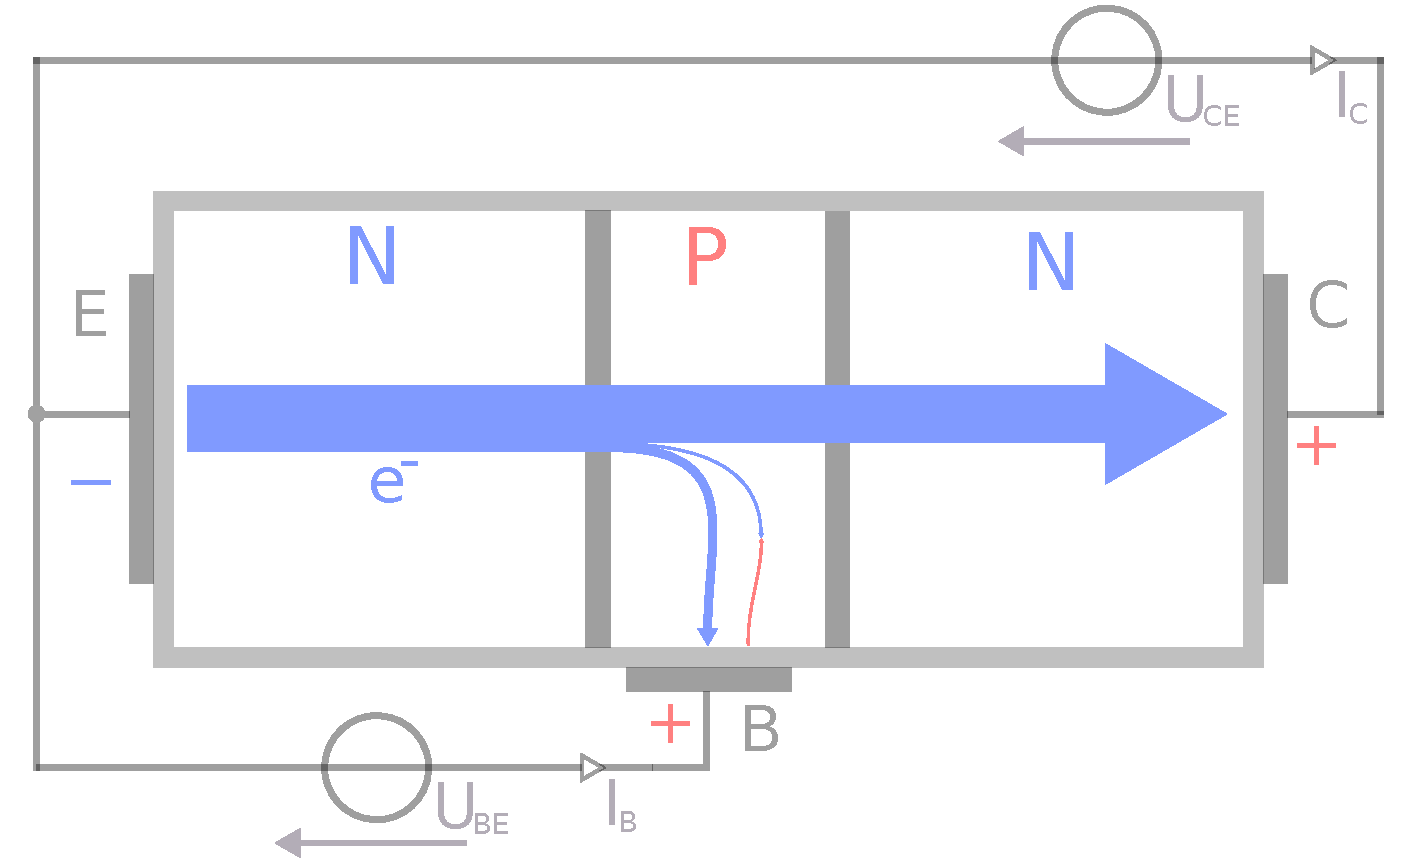
\includegraphics[width=0.618\textwidth]{1_1/npn_voltage_both.pdf}
  \end{center}
\end{figure}
Legt man eine zusätzliche Spannung an die Kollektor-Emitter-Strecke, so ist das elektrische Feld der Raumladungszone des Basis-Kollektorübergangs so gerichtet, dass sich die Elektronen des Emitters in Richtung Kollektor bewegen (Drift). Außerdem rekombinieren diese nicht in der Basis, da die Basisweite sehr gering ist. Es fließt ein Elektronenstrom zwischen Kollektor und Emitter, der durch einen deutlich geringeren Basisstrom gesteuert wird.


%%%%%%%%%% Ebers Moll
Ein mathematisches Modell zur Beschreibung des statischen Verhaltens des Bipolartransistors bietet das \emph{Ebers-Moll-Modell}:

\begin{center}
\begin{circuitikz}
  \draw (-1,0) to [short, o-, i<=$I_E$] (0,0);
  \draw (2,0) to [diode, v=$I_{ED}$] (0,0);
  \draw (2,0) to [diode, v^=$I_{CD}$] (4,0);
  \draw (4,0) to [short, -o, i<=$I_C$] (5,0);
  \draw (1.5,0) to [short] (2.5,0);
  \draw (2,0) to [short, *-o, i<^=$I_B$] (2,-2);
  \draw (0,0) to [short, *-] (0,2);
  \draw (2,0) to [short, *-*] (2,2);
  \draw (4,0) to [short, *-] (4,2);
  \draw (4,2) to [current source, l_=$A_N \cdot I_{ED}$, i=$$] (2,2);
  \draw (0,2) to [current source, l=$A_I \cdot I_{CD}$, i=$$] (2,2);
  \node[left] at (-1,0) {E};
  \node[right] at (5,0) {C};
  \node[below] at (2,-2) {B};
\end{circuitikz}
\end{center}

Knotengleichung am Emitter:

\[ I_E = I_{ED} - A_I \cdot I_{CD} \]
\[ I_E = I_{ES} \cdot \left( e^{\frac{U_{BE}}{U_T}} - 1 \right) - A_I \cdot I_{CS} \cdot \left( e^{\frac{U_{BC}}{U_T}} - 1 \right) \]

Knotengleichung am Kollektor:
\[ I_C = I_{CD} - A_N \cdot I_{CD} \]
\[ I_C = I_{CS} \cdot \left( e^{\frac{U_{BC}}{U_T}} - 1 \right) - A_N \cdot I_{ES} \cdot \left( e^{\frac{U_{BE}}{U_T}} - 1 \right) \]

Basis:
\[I_B = I_E - I_C\]
\[I_B = (1-A_N) \cdot I_{ES} \cdot \left( e^{\frac{U_{BE}}{U_T}} -1\right) - (1-A_I) \cdot I_{CS} \cdot \left( e^{\frac{U_{BC}}{U_T}} -1\right)\]


Im Normalbetrieb (Basis-Emitter-Übergang in Durchlass-, Basis-Kollektor-Übergang in Sperrrichtung) können die inversen Anteile des Modells vernachlässigt werden und es vereinfacht sich zu:
\begin{center}
\begin{circuitikz}
  \draw (-1,0) to [short, o-, i<=$I_E$] (0,0);
  \draw (2,0) to [diode, v=$I_{ED}$] (0,0);
  \draw (4,0) to [short, -o, i<=$I_C$] (5,0);
  \draw (2,0) to [short, *-o, i<^=$I_B$] (2,-2);
  \draw (2,0) to [short, -] (2,2);
  \draw (4,0) to [short, -] (4,2);
  \draw (4,2) to [current source, l_=$A_N \cdot I_{ED}$, i=$$] (2,2);
  \node[left] at (-1,0) {E};
  \node[right] at (5,0) {C};
  \node[below] at (2,-2) {B};
\end{circuitikz}
\end{center}
\[I_E = I_{ED}\] 
\[I_C = A_N \cdot I_{E}\] 
\[I_B = \frac{1-A_N}{A_N} \cdot I_{C}\] 

